\section{Main simulator panel}
    This panel is the main part of the simulator user interface. Simulator mimics functionality of PicoBlaze instruction set and provide detailed view in its registers, overview of input and output ports, etc., and displays warning when the simulated program behaves strangely i.e. does something which under normal circumstances results an error. Following picture shows main window of the simulator. You can find here internal registers, scratch-pad ram, input and output ports, stack, program counter, elapsed time and cycles, current clock and internal flags: carry and zero. All those features can be edited during processor simulation. If some value changes state, it will turn yellow. You can drag out whole simulation panel and place outside of the main window, for example another display on your computer.

   \begin{figure}[h!]
        \centering
        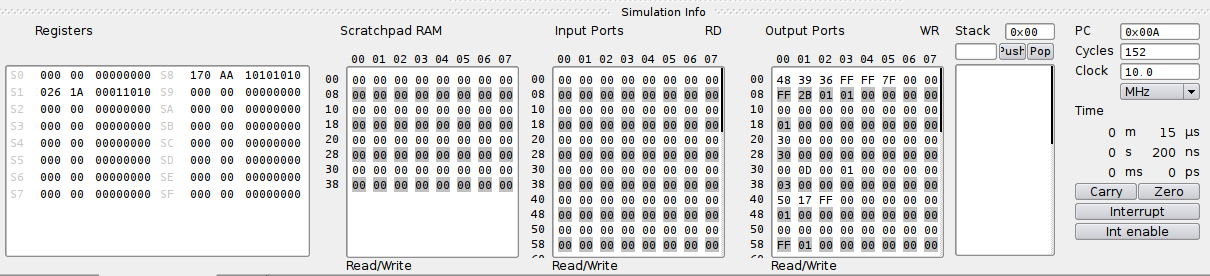
\includegraphics[width=\textwidth]{img/bottom_panel.png}
        \caption{Main simulator panel}
    \end{figure}

    \begin{description}
        \item [Registers]
            You can find here values of internal processor registers. The first column represents name, second value in decimal, third hexadecimal value, and last binary value.
        \item [Scratch-pad RAM]
            This hexadecimal editor represents values stored in the scratch-pad RAM. Address of a particular field is addition of the line and column numbers.
        \item [Ports]
            Output and input ports are represented by hexadecimal editors in their full address range. Besides viewing and changing input and output values, you can also see the status of PicoBlaze RD, WR, and WRK signals (read and write strobes).
        \item [Stack]
            Stack window represents values stored in stack. You can change the stack content by pushing and popping values, and view its virtual stack pointer.
        \item [Info panel]
            Panel on the right side of simulation panel gives you general information about simulated code. You can find there the program counter, number of executed cycles, clock frequency, elapsed time and status flags Carry and Zero, plus normally hidden Interrupt Enable flag. You can also invoke an interrupt by clicking on the Interrupt button. Buttons showing status flags or other flags can also change them (click on such button to invert the flag). Green text in ``flag button'' indicates that the flag is set to 1, black text indicates that value of the flag is 0.
    \end{description}

    \subsection{Modes of simulation}
        The simulator can operate three different modes:
        \begin{description}
            \item [Step]
                \index{Step mode}
                Step by step simulation, executes only one instruction when invoked, no matter how many machine cycles it will take (this does not apply for macro-instruction, in that case each instruction of the macro is executed separately).
            \item [Animation]
                \index{Animation mode}
                Similar to the step mode but in a loop, instructions are executed one after another until stopped on user request, or by a simulator waring message.
            \item [Run]
                \index{Run mode}
                Run is generally the same as animation but much faster, GUI is not updated so often, and changes in the registers, ports, etc. are not shown until the run is halted.
        \end{description}

    \subsection{Simulator warnings}
        The simulator can display several warnings to handle some common mistakes in software development like program counter overflow, stack overflow, and some others; it is meant to make your debugging process less painful. To adjust settings related simulator warnings, please go to [Main~Menu]~-> [Interface]~-> [Configure]~-> [Simulator~warnings].

        \subsubsection{Simulator warning groups}
        \begin{description}
            \item[Memory]~\\
                The memory group relates to suspicious and invalid attempts to access program memory, register file, scratch-pad memory, and even ports of the simulated processor.
            \item[Stack]
                The stack group is related to processor call stack.
            \item[CPU]
                The CPU group contains warnings related control flow and interrupt handling.
        \end{description}

    \clearpage
    \subsection{Simulation cursor}
        Simulation cursor shows what instruction will be executed in next step. Two previously executed instructions are highlighted but with lower and fading intensity; you can use that to easier track previous steps. Following figure shows actual cursor on line 8, one step before is on line 5, and two steps before is on 4.
        \begin{figure}[h!]
            \centering
            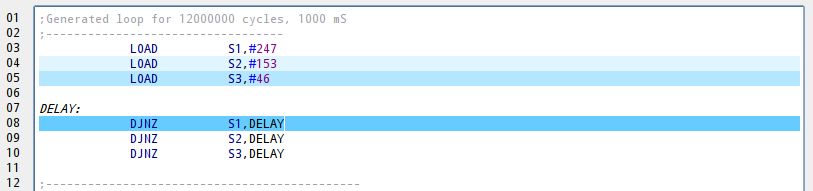
\includegraphics[width=\textwidth]{img/simulationcursor1.png}
            \caption{Simulation cursor}
        \end{figure}

        When simulator encounters macro expansion, for better orientation, cursor will appear on two or more locations. On macro expansion and in macro definition, showing what is being executed and where it came from. When you have macro expanded in another macro, you will see three cursors and so on. For better understanding, the following figure shows simulation cursor behavior with macros.
        \begin{figure}[h!]
            \centering
            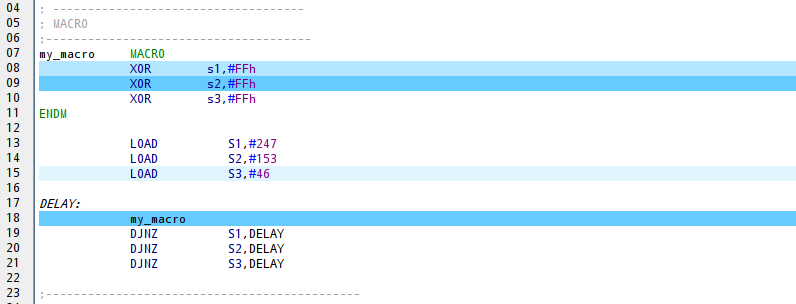
\includegraphics[width=\textwidth]{img/simulationcursor2.png}
            \caption{Simulation cursor (with macros}
        \end{figure}
